\section{\texorpdfstring{Architektura MCU}{Architektura MCU}}

% =====================================================================================================================
	\begin{frame}
    \frametitle{Číslicový počítač - velmi krátká historie}
		
		
		\begin{center}
			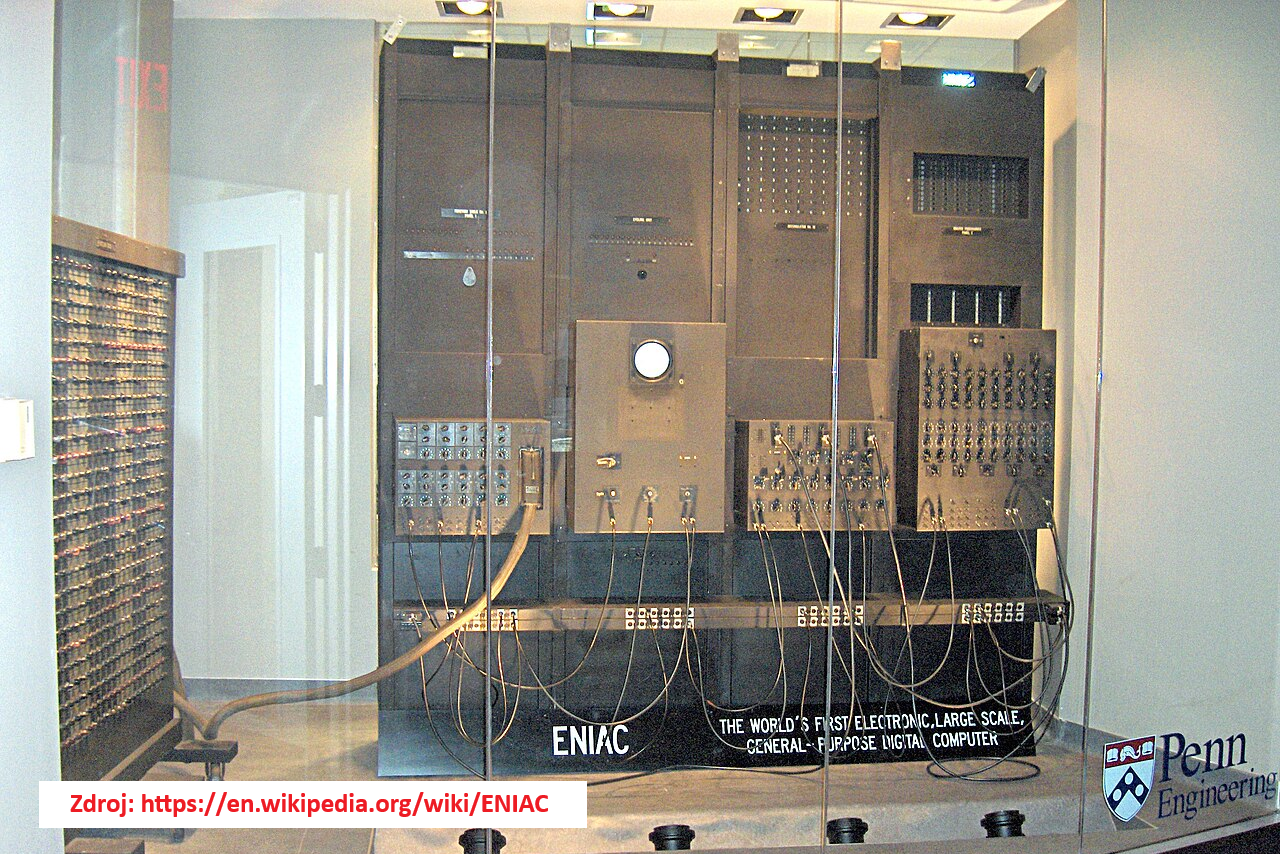
\includegraphics[width=0.48\textwidth]{fig/ENIAC.png}
		\end{center}
	
		\begin{itemize}
			\item 60. léta velké sálové počítače,
			\item 70. léta nástup mikroprocesorové techniky,
			\item 80. léta osobní počítače,
			\item 90. léta internet, počítačové sítě,
			\item dnes: osobní počítače, řídicí počítače (vestavné), superpočítače.
	
		\end{itemize}
	\end{frame}
	
% =====================================================================================================================
	\begin{frame}
    \frametitle{Číslicový počítač - nedílné části}
		
		
		\begin{center}
			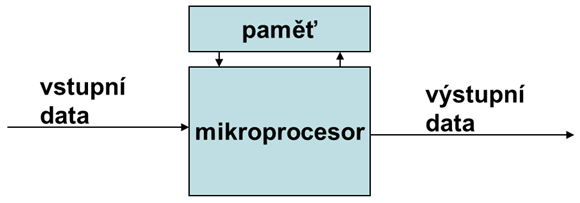
\includegraphics[width=0.5\textwidth]{fig/computer_basic_parts.png}
		\end{center}
		
		\begin{itemize}
			\item \textbf{Mikroprocesor:}
			
			\begin{itemize}
				\item ALU,
				\item řídicí obvody,
			\end{itemize}
			
			\item \textbf{Paměť:}
			
			\begin{itemize}
				\item nahrávání / ukládání programu,
				\item ukládání dat (proměnné).
			\end{itemize}
			
		\end{itemize}
		
		\vspace{2mm}
		\textbf{POZN.}: Kromě číslicového počítače existují i analogové počítače, které se dříve používaly pro simulace fyzikálních dějů.

	\end{frame}
	
% =====================================================================================================================
	\begin{frame}
    \frametitle{Číslicový počítač - Architektura}
		
		\textbf{Architektura:} zde je to konkrétní struktura a uspořádání jednotlivých prvků počítače a jejich propojení, můžeme ji dělit například
		
		
		\begin{itemize}
			\item podle přístupu k paměti na Harvardskou a von Neumannovu,
			\item podle instrukční sady na RISC a CISC,
			\item podle velikosti základní datové jednotky (v podstatě základní šířka registrů) na 8, 16, 32 bitovou atd.
		\end{itemize}
		
		\vspace{3mm}
		\textbf{Procesor STM8S208RB:}
		\begin{itemize}
			\item modifikovaná Harvardská architektura,
			\item CISC,
			\item 8 bitů.
		\end{itemize}

	\end{frame}
	
% =====================================================================================================================
	\begin{frame}
    \frametitle{Číslicový počítač - von Neumannova architektura}
		
		\small
		\begin{center}
			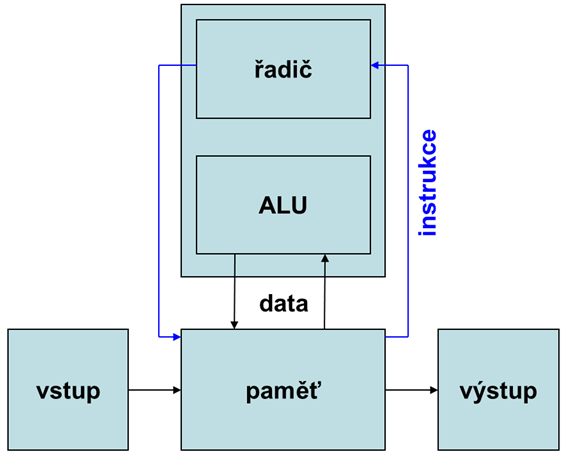
\includegraphics[width=0.4\textwidth]{fig/arch_vonNeumann.png}
		\end{center}
		
		
		\begin{itemize}
			\item Sdílená sběrnice pro data i program,
			\item lze adresovat stálá data (tabulky) v programové paměti,
			\item zpracování instrukcí je rychlejší než přístup k paměti $\Rightarrow$ vzniká omezení rychlosti dané rychlostí paměti,
			\item zpomalení částečně kompenzuje paměť CACHE. 
		\end{itemize}

	\end{frame}
	
% =====================================================================================================================
	\begin{frame}
    \frametitle{Číslicový počítač - Harvardská architektura}
		
		\small
		\begin{center}
			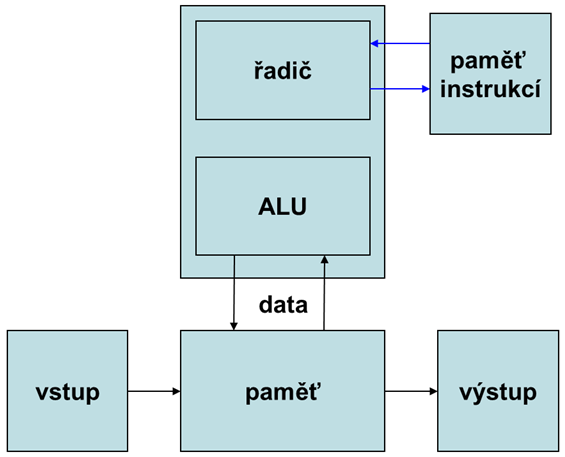
\includegraphics[width=0.4\textwidth]{fig/arch_Harvard.png}
		\end{center}
		
		
		\begin{itemize}
			\item Oddělená sběrnice pro data a program,
			\item \textcolor{red}{\textbf{ne}}lze adresovat data v programové paměti, pokud neexistuje vhodná modifikace,
			\item načtení další instrukce lze do určité míry dělat současně se zápisem nebo čtením dat.
		\end{itemize}

	\end{frame}
	
% =====================================================================================================================
	\begin{frame}[fragile]
    \frametitle{Číslicový počítač - modifikovaná Harvardská architektura}
		
		Případ procesoru \textbf{STM8S208RB:}
		
		\begin{itemize}
			\item Používá jednotný paměťový prostor (Unified Memory),
			\item díky tomu lze adresovat jak paměť dat, tak paměť programu,
			\item načtení další instrukce lze do určité míry dělat současně se zápisem nebo čtením dat.
		\end{itemize}
		
		\vspace{3mm}
		To umožňuje zápis následujícího kódu v jazyce C:
		\hrule
		\footnotesize
		\begin{lstlisting}[language=C]
	const int moje_konstanta = 314; // FLASH
	int moje_promenna = 200;        // RAM

	moje_promenna = moje_promenna + moje_konstanta;
		\end{lstlisting}
		
		\hrule
		\textbf{Příklad problému pro mcu AVR Atmel (ARDUINO):} označení \textbf{const} umisťuje hodnotu stále do paměti RAM. Pro umístění do FLASH musíte používat příslušná makra knihovny \textbf{\uv{avr/pgmspace.h}}.
	\end{frame}

% =====================================================================================================================
	\begin{frame}
    \frametitle{Číslicový počítač - paměť}
		
		\begin{minipage}[t][\textheight][t]{0.5\textwidth}
		\small
		\begin{itemize}
			\item Data:
			
			\begin{itemize}
				\item čísla - daná velikostí buňky,
				\item znaky - dle kódování např. ASCII.
			\end{itemize}
			
			\item Organizace:
			
			\begin{itemize}
				\item paměťová buňka
				\item po bytech, slovech, ... 
			\end{itemize}
			
			\item Zarovnání \uv{širších} hodnot:
			
			\begin{itemize}
				\item \textbf{Big Endian} - začíná největším koncem (řádem, bytem, bitem)
				\item \textbf{Little Endian} - začíná nejmenším koncem (řádem, bytem, bitem)
			\end{itemize}
		\end{itemize}
	
		\end{minipage}
		\begin{minipage}[t][\textheight][t]{0.45\textwidth}
		Zápis 16 bit hodnoty \textcolor{blue}{\textbf{0x4321}}:
		
		\vspace{2mm}
		\textbf{Big Endian}
		
		\begin{center}
			\begin{tabular}{| r | c |}
				\hline
				\textbf{Adresa} & \textbf{Data} \\
				\hline
				0x000001 & 0x43 \\
				\hline
				0x000002 & 0x21 \\
				\hline
			\end{tabular}
		\end{center}
		
		\vspace{2mm}
		\textbf{Little Endian}
	
		\begin{center}
			\begin{tabular}{| r | c |}
				\hline
				\textbf{Adresa} & \textbf{Data} \\
				\hline
				0x000001 & 0x21 \\
				\hline
				0x000002 & 0x43 \\
				\hline
			\end{tabular}
		\end{center}
		
		\end{minipage}
		
	\end{frame}
	
% =====================================================================================================================
	\begin{frame}
    \frametitle{Číslicový počítač - datová komunikace}
		
		
		\begin{center}
			
\includegraphics[width=0.70\textwidth]{fig/bus.png}
		\end{center}
		
		
		\begin{itemize}
			\item Všechny bloky jsou spojeny sběrnicemi:
			
			\begin{itemize}
				\item adresová - adresace konkrétního bloku,
				\item datová - přenos dat,
				\item řídicí - řízení komunikace na sběrnici.
			\end{itemize}
			
			\item Do adresového rozsahu náleží i registry periférií - stejná sběrnice.
		\end{itemize}
		
	\end{frame}

% =====================================================================================================================
	\begin{frame}
    \frametitle{Číslicový počítač - sběrnicový systém}
		
		\begin{minipage}[t][\textheight][t]{0.8\textwidth}
		
		\textbf{Příklad:}
		\begin{center}
			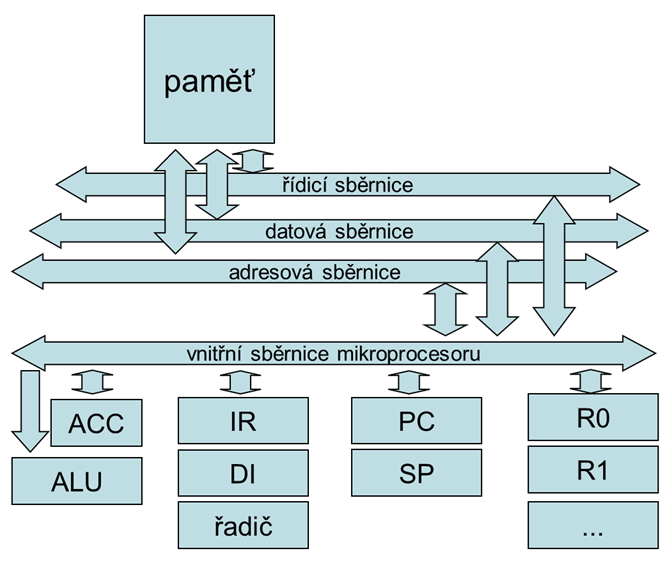
\includegraphics[width=0.80\textwidth]{fig/bus_system.png}
		\end{center}
			
		\end{minipage}
		\begin{minipage}[t][\textheight][t]{0.12\textwidth}
		\tiny
		\begin{center}
		\textbf{STM8}
			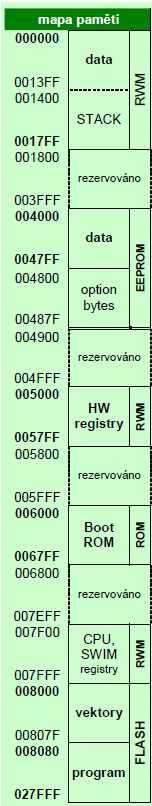
\includegraphics[width=0.9\textwidth]{fig/memory_STM8.png}
		\end{center}
		
		\end{minipage}
		
	\end{frame}
	
% =====================================================================================================================
	\begin{frame}[fragile]
    \frametitle{Číslicový počítač - CISC vs RISC}
		
		\begin{minipage}[t][\textheight][t]{0.48\textwidth}
		\textbf{CISC:}
		
		\begin{itemize}
			\item složité instrukce,
			\item obvykle proměnná délka instrukce,
			\item komplexní operace v jedné instrukci,
			\item v rámci instrukce umožňuje různé způsoby adresování,
			\item jednodušší pro programátora.
		\end{itemize}
		
		\vspace{2mm}
		\textbf{STM8}
		\footnotesize
		\begin{lstlisting}
	ld   A, var1
	add  A, var2
	ld   var3, A
		\end{lstlisting}
		
		\end{minipage}
		\begin{minipage}[t][\textheight][t]{0.48\textwidth}
		\textbf{RISC:}
		\begin{itemize}
			\item jednoduché instrukce,
			\item často stejná délka instrukce,
			\item jednoduché kroky:\\
			nejjednodušší příklad je násobení řešené pomocí instrukce pro sčítání. 
		\end{itemize}
		
		\vspace{2mm}
		\textbf{ARM Cortex-M}
		\footnotesize
		\begin{lstlisting}
	ldr r1, =var1
	ldr r3, =var2
	ldr r4, =var3
	ldr r0, [r1]
	ldr r2, [r3]
	add r0, r0, r2
	str r0, [r4]
		\end{lstlisting}
		\end{minipage}

	\end{frame}